\documentclass[conference]{IEEEtran}
% \IEEEoverridecommandlockouts
% The preceding line is only needed to identify funding in the first footnote. If that is unneeded, please comment it out.
\usepackage{cite}
\usepackage{amsmath,amssymb,amsfonts}
\usepackage{algorithmic}
\usepackage{graphicx}
\usepackage{textcomp}
\usepackage{xcolor}
\usepackage{url}


\begin{document}

\title{Single Image Dehazing}

\author{\IEEEauthorblockN{Arico Amaury}
\IEEEauthorblockA{\textit{BruFace student}}
\and
\IEEEauthorblockN{Colot Emmeran}
\IEEEauthorblockA{\textit{BruFace student}}
\and
\IEEEauthorblockN{Khansir Nima}
\IEEEauthorblockA{\textit{BruFace student}}}

\maketitle

\begin{abstract}
Outdoor images are affected by atmospheric visibility reduction, particularly haze. The hazing effect is influenced by several 
factors including location, weather, pollution level and other geographic and environmental parameters. Visibility degradation depends on the distance between the camera and the scene points. Literature shares various algorithms to dehaze outdoor 
images.  As part of the image processing project, our group will apply an algorithm performing a dehazing process requiring
one single input developed by scientists from Hebrew University of Jerusalem \cite{airlight} \cite{dehaze}. By delimiting and exploiting local patches from this single input, the global airlight vector - the atmospheric
colour - and the transmission gradient - the hazing reduction coefficient - are extracted.  Through this report, we will describe 
the three steps of the algorithm, validate the dehazing process by showing the after-process results and compare it with the 
original pictures.  
\end{abstract}

\section{Introduction}

Haze, visibility reduction phenomenon, is coming from the presence in the atmosphere of particles scattering the ambient 
light, attenuating the contrast for outdoor images and corrupting the true radiance of the scenery by a ambient colour.
Most dehazing algorithms are performed based on the RGB representation of the images.
The haze effect is commonly modelled by the following equation \cite{airlight}:

\begin{equation}
\label{image_model}
\mathbf{I}(\mathbf{x}) = t(\mathbf{x}) \mathbf{J}(\mathbf{x}) + (1-t(\mathbf{x})) \mathbf{A}
\end{equation}

where $\mathbf{x}$ is the pixel position, $\mathbf{I}$ is the pixel colour under hazing condition or in other words, the image input, $\mathbf{A}$ is the ambient light colour,
$\mathbf{J}$ the true pixel radiance, $t$ is the transmission coefficient ranging from 0 (airlight colour)
to 1 (true colour), which is distance-dependent. It is defined by \cite{dehaze} as:

\begin{equation}
\label{scattering_coefficient}
t(\mathbf{x}) = e^{-\beta d(\mathbf{x})}
\end{equation}

where $\beta$ is the wave phase number and $d(\textbf{x})$ the scene pixel distance from the camera.  From equation (\ref{scattering_coefficient}),
one can observe $t(\mathbf{x})$ is dependent on the wavelength and is thus different for each colour component.  Nevertheless, the used algorithm assume a constant matting gradient $t(\mathbf{x})$ for each colour channel.
The contrast attenuation and the ambient colour corruption can be highlighted by breaking the equation (\ref{image_model}) in two distinct parts: 
\begin{itemize}
    \item $t(\mathbf{x}) \mathbf{J}(\mathbf{x})$, the true radiance component,
    \item $(1-t(\mathbf{x})) \mathbf{A}$, the ambient light effect.
\end{itemize}
$\mathbf{I}(\mathbf{x})$ being the input image, the dehazing process is reduced to find the transmission and the global airlight parameters to recompose
the true radiance scenery.  This process can be decomposed in three steps : determining the airlight vector direction, finding its magnitude and finally computing the transmission coefficient.

\section{Airlight vector determination}  

Even if the algorithm is indeed based on the equation (\ref{image_model}), it uses a reformulation of it \cite{airlight}:

\begin{equation}
\label{shading_coefficient}
\mathbf{I}(\mathbf{x}) = l(\mathbf{x}) \mathbf{R}_i + c_i \mathbf{A}
\end{equation}

Where $l(\mathbf{x})$ expresses the shading coefficient related to the angle between the normal direction of the scene surface and
the light source direction, $R_i$ is the true radiance and $c_i$, the ambient light coefficient $(1-t(\mathbf{x}))$.
The airlight determination method described in \cite{airlight} is a local patch-based algorithm meaning the image is decomposed on patches on which information is
gleaned after image treatment.  The patches should obey to specific conditions : it should be composed of pixels with same
true radiance and with constant transmission coefficient. In other words, the patches are composed of pixel of same true colour and affected
by the same haze intensity effect. The motivation behind this decomposition lies in the retrieval of the airlight
vector.  By finding patches composed of pixels fulfilling the previous constraints, we gather group of pixels with colour magnitude
varying in function of the coefficient $l(\mathbf{x})$ - function of the normal direction of the surfaces/pixels.  By representing these pixels in the RGB 3D space, it is possible to construct, for each patch, the line $\mathbf{I}(\mathbf{x}) = l(\mathbf{x}) \mathbf{R}_i + \mathbf{C}$ 
with $\mathbf{C}$ a constant equals to $c_i \mathbf{A}$ ($c_i$ assumed to be constant in the patch area considering the smoothness of the scene radiance for outdoor pictures).
The funding idea of the algorithm is that the constructed line will intersect the airlight vector in the RGB space when $l(\mathbf{x}) = 0$.
Constructing planes formed by the patches lines passing by the origin and intersecting the planes by pairs will lead to the
determination of the airlight vector candidates which ultimately will result to the dehazing of the image.

The importance of the airlight vector has been introduced in the introduction and we will now move to its computation.
the first part will be focused on the determination of the orientation of the airlight vector - the magnitude calculation is done 
in the second part of the algorithm. The vector orientation can be calculated in 7 steps:
\begin{itemize}[\IEEEsetlabelwidth{vi}]
\item[i] \textit{Patch decomposition} As mentioned previously, the airlight vector can be calculated through local patches processing. 
Thus the initial step is to generate these local patches from the image. The size of those patches is set to $10 \times 10$ pixels, which leads to optimal results for most cases \cite{airlight}. Only patches with smooth variations
should be kept avoiding rough colour distortion within a patch which will affect the colour line vector calculation.  Therefore, Canny
algorithm is run upstream detecting patches with edges and getting rid of them for next steps.
\item[ii] \textit{Main principal component analysis} The construction of the patch lines, or patch vectors, are calculated by computing the principal component analysis (PCA) resulting to the eigenvectors computation and their
associated eigenvalues.  The patch vectors are defined by the largest PCA with its origin at the centroïd of the patch pixels.
The PCA is performed 2 times to be exact.  We construct first the patch line by considering all the pixels and aftewards the 20 \% farthest
pixels from the first estimated line are discarded and we recompute the vector.  
\item[iii] \textit{Eigenvalue comparison} Once the first filter with Canny has been applied and the patches lines have been computed, 
a second filtering is performed.  To ensure that the patch lines are resulting from a collection of pixel showing a 1D variability 
along the variation of the shading coefficient $l(\mathbf{x})$, we set threshold regarding the main eigenvalue.
First the main eigenvalue should be higher than a threshold $\tau_1$ ensuring being high enough - $\lambda_1 > \tau_1$. 
Secondly, the ratio between the main eigenvalue and the sub ones should be higher than a threshold $\tau_2$ - $\frac{\lambda_1}{\lambda_2} > \tau_2$ - 
ensuring a high linearity.
\item[iv] \textit{Distance to origin} After collecting patch lines with a high main PCA, we need to ensure that the patch lines 
comply with another criteria related to the distance from the patch vector and the origin of RGB space.
If the eigenvector passes by the origin or close to the origin, it would mean that the pixels within the patches would be not 
affected by the global airlight and thus would not contain valuable information to reconstruct the airligth vector.  
The distance from the origin should therefore be higher than a threshold $\tau_3$.  The distance from the eingenvector to the origin
can be computed through the cross product as follow.

\begin{equation}
\label{Distance to origin}
dist_{0,0} = \frac{||\vec{v_{eig}} \times \vec{\mu}||}{||\vec{v_{eig}}||}
\end{equation}

where $v_{eig}$ is the eigenvector and $\mu$ the centroid of the pixels withtin the local patch.
Additional filtering should be done to ensure that all the valid pacthes eigenvector contains only non negative components being 
not representative of outdoor reflective light $l(x)R_i$.

\item[v] \textit{Eigenvector angles threshold} Finally, we need to discard the patch leading to similar patch lines which would result 
to wrong airlight vector candidates computation in point vi.  To ensure no false result, the angle between two patch lines 
should be above $15 \deg$ [1].
\item[vi] \textit{Airlight candidates computation}  After patches validation, we can now compute the airlight vector candidates.
We first construct the plane defined with the patch vector and passing by the origin.  Once the planes are defined for each patch, each pair of planes 
 intersection are calculated and defines airlight vector candidates :

\begin{equation}
\label{Normal_vector}
\vec{n_i} = \vec{v_{eig_i}} \times \vec{\mu_i}
\end{equation}

\begin{equation}
\label{airlight_candidate}
\vec{\text{Â}}_{cand} = \frac{\vec{n_i} \times \vec{n_j}}{||\vec{n_i} \times \vec{n_j}||} 
\end{equation}

where $n_i, n_j$ are normal vector from the {centroid x patch line} plane and $\text{Â}_{cand}$ the airlight vector.
\item[vii] \textit{Minimal distance for  determination} Finally, each potential airlight candidate is compared by 
computing the Euclidian distance between the considered candidate and the patch lines.  The lowest median distance candidate is selected as 
the best fit vector.  Mathematically, it gives the equation (\ref{airlight_vector}).

\begin{equation}
\label{airlight_vector}
\vec{\text{Â}}_{vector} = argmin_j(median_i(d_{ij})) 
\end{equation}

where $d_{ij}$ is the Euclidian distance between the $j$-th airlight candidate $\text{Â}_{cand}$ and the $i$-th patch line.
\end{itemize}   

Regarding the threshold $\tau_1, \tau_2, \tau_3$ values, they are initiated to keep more than 10 patches and are afterwards refined by increasing step
by step the thresholds until 10 patches remain.  These patches are used for the airlight candidates computation at the point vi.

\section{Airlight magnitude determination}
%%%%%%%%%%%%%%%%%%%%%%%%%
In the continuity of recovering the clear scene radiance \( J(x) \) from a hazy image \( I(x) \), it is essential to determine the full atmospheric light vector \( A = \|A\|\hat{A} \). 
Indeed, once the orientation of the atmospheric light vector has been found, we use the method described in \cite{airlight} to derive the airlight amplitude. The airlight being closely related to pixel brightness and transmission, estimating it will be more complex. The key idea is to exploit the empirical regularity that in natural hazy scenes, the brightness of the brightest pixels tends to be independent of their transmission. This regularity allows us to formulate an optimization procedure to estimate \( \|A\| \) robustly.

\subsection{Initial Dehazing with Unit Amplitude}

We begin by applying a dehazing function assuming a unit amplitude, i.e., \( \|A\| = 1 \). This provides an initial estimate of the transmission map \( t(x) \) and the dehazed image \( J(x) \).To analyze how image brightness varies with transmission, we compute a scalar brightness value \( l(x) \) at each pixel of the initially dehazed image \( J(x) \). This is done by taking the Euclidean norm of the RGB vector:
\begin{equation}
\label{initial_brightness }
l(x) = \|J(x)\|_2 = \sqrt{J_R(x)^2 + J_G(x)^2 + J_B(x)^2}
\end{equation}

This is justified by the scene radiance model assumed in \cite{airlight}, where the dehazed image is decomposed as \( J(x) = l(x) R(x) \), with \( R(x) \) being the chromaticity (i.e., a unit-norm color vector) and \( l(x) \) being the scalar brightness. Since \( \|R(x)\|_2 = 1 \), it follows that \( \|J(x)\|_2 = l(x) \). Thus, taking the 2-norm of each pixel vector in \( J(x) \) directly recovers the brightness component. This brightness estimate plays a central role in constructing the percentile-based brightness statistic used later to estimate the airlight amplitude.
%%%%%%%%%%%%%%%%%%%%%%%%%%%%%%%%%%%%%%%%%%



%%%%%%%%%%%%%%%%%%%%%%%%%%%%%%%%%%




\subsection{Max-Brightness Invariance Statistic}
Based on the per-pixel brightness \( l(x) \), we compute a transmission-dependent brightness statistic denoted by \( l^*_a(s) \). This function represents the 99th percentile of the brightness values \( l(x) \) among pixels that share a similar transmission value \( s \) \cite{airlight}. The motivation for using this statistic stems from a global regularity observed in natural hazy images \cite{airlight}: the brightness of the brightest pixels tends to remain approximately invariant across different transmission levels.
\begin{equation}
\label{brightness_statistic}
l^*_a(s) = \text{percentile}_{99\%} \{ l(x) \mid t(x) = s \}
\end{equation}
To construct \( l^*_a(s) \), we begin by uniformly dividing the transmission range \([0, 1]\) into a fixed number of bins. Each bin is associated with a central transmission value \( s \). For each bin, we collect all pixels whose estimated transmission \( t(x) \) falls within a small interval centered around \( s \). Among these pixels, we extract the 99th percentile of the corresponding brightness values \( l(x) \). This process yields a curve \( l^*_a(s) \), which captures how the brightness of the brightest pixels varies as a function of transmission.

In theory, if the correct atmospheric light magnitude \( \|A\| \) is used, this curve should be nearly flat, since the multiplicative brightness bias introduced by an incorrect \( \|A\| \)  would otherwise distort the brightness of the dehazed image depending on transmission. Thus, deviations from flatness in \( l^*_a(s) \) serve as a cue for detecting and correcting such amplitude errors. This principle underlies the subsequent optimization used to recover the correct airlight amplitude.

\subsection{Optimization to Recover Amplitude}

Assuming that the correct airlight amplitude yields a flat \( l^*_a(s) \), we define a cost function based on a theoretical transformation of transmission and brightness that occurs when using a wrong amplitude. The derivation of this transformation relies on a key assumption presented in the paper \cite{airlight} : even if the wrong amplitude \( \hat{a} \cdot \hat{A}\) is used in dehazing, the method still attempts to match the true airlight term, i.e.,

\begin{equation}
\label{matching_airlight}
(1 - t_a(x)) \cdot aA = (1 - t(x)) \cdot A
\end{equation}

This assumption ensures preservation of the additive haze (airlight) component across different amplitude choices. Solving this equation for \( t_a(x) \), the transmission recovered under an incorrect amplitude, yields:

\begin{equation}
\label{recovered_transmission }
t_a(x) = \frac{t(x) - 1}{a} + 1
\end{equation}

However, since the transmission and radiance must still balance the full image formation equation, this mismatch introduces a brightness bias into the recovered dehazed image. As shown in \cite{airlight}, this bias is captured in by a transmission-dependent factor:

\begin{equation}
\label{brightness_bias}
\sigma_a(t) = \frac{a t}{t + a - 1}
\end{equation}

To recover the correct amplitude \( \hat{a} = \|A\| \), we minimize the squared error between the observed brightness statistic \( l^*_a(s) \) and the predicted scaled brightness \( \sigma_a(s) \cdot k \), using:

\begin{equation}
\label{optimisation}
\min_{\hat{a}, k} \sum_s \left( l^*_a\left( \frac{s - 1}{\hat{a}} + 1 \right) - \sigma_\hat{a}(s) \cdot k \right)^2
\end{equation}

This non-linear least-squares problem is solved using numerical optimization. The optimal value of \( a \) is then used to reconstruct the full atmospheric light vector as \( A = a \cdot \hat{A} \).


\subsection{Robustness and Final Estimation}
%%%%%%%%%%%%%%%%%%%%%%%%%%%%%%%%%%%%%%%%%%


%%%%%%%%%%%%%%%%%%%%%%%%%%%%%%%%%%
During optimization, we apply a remapping of transmission values defined by \( s_a = \frac{s - 1}{a} + 1 \). However, for small values of \( a \), this mapping can produce negative transmission levels \( s_a < 0 \), which are physically invalid and lead to undefined behavior during percentile interpolation. To address this, a correction step is implemented \cite{airlight}: if any remapped transmission value becomes negative, we slightly increase the norm of the airlight orientation vector \( \hat{A} \). This effectively raises the estimated airlight magnitude used during the initial dehazing, producing new estimates of \( J(x) \), \( t(x) \), and \( l^*_a(s) \) that are more stable. The optimization is then re-run with these updated statistics until all remapped values are valid. This step ensures the cost function remains well-defined over the domain of transmission bins.

Finally, the estimated amplitude \( \hat{a} \) is multiplied by the orientation to form the complete atmospheric light vector:

\begin{equation}
\label{airlight}
A = \hat{a} \cdot \hat{A}
\end{equation}

This estimation is crucial for ensuring that the dehazed image does not suffer from brightness artifacts related to incorrect atmospheric light scaling.

\section{transmission range determination}
The method described in \cite{dehaze} is based on a simple assumption: an image without any haze is often composed of a few dominant colours. This allows to regroup the pixels of the input image in a few clusters, each representing one of those dominant colours. Each pixel inside such cluster will be, according to Eq. (\ref{image_model}), between the dominant colour and the airlight vector determined previously. The transmission coefficient can then be computed by finding the distance between the pixel and the airlight vector.\par
The clusters described previously are named \textit{haze-lines} in \cite{dehaze}. and are found by first centering the image around the airlight vector:
\begin{equation}
    \label{eq:centered_image}
    \mathbf{I}_A(\mathbf{x}) = \mathbf{I}(\mathbf{x}) - \mathbf{A}
\end{equation}
This means that, when combined with Eq. (\ref{image_model}):

\begin{equation}
    \label{eq:centered_image_model}
    \mathbf{I}_A(\mathbf{x}) = t(\mathbf{x}) \left[\mathbf{J}(\mathbf{x}) - \mathbf{A}\right]
\end{equation}

And this centered image is then represented in polar coordinates. This means that each pixel x will be represented by its distance to the airlight vector and its longitudinal and azimuthal angle with respect to it:
\begin{equation}
    \label{eq:polar_coordinates}
    \mathbf{I}_A(\mathbf{x}) = \left[r(\mathbf{x}), \theta(\mathbf{x}), \phi(\mathbf{x})\right]
\end{equation}

In this polar system, pixels with a similar orientation belong to the same haze-line as they would then all have a color between the airlight vector and the dominant color of the haze-line. The clustering is performed by splitting the polar coordinates into 1000 bins (done by the authors of \cite{dehaze} in \cite{github}) and then finding the nearest bin for every pixel. Fig. \ref{fig:haze_lines} shows one of the haze-lines together with the reference image. 
\begin{figure}
    \centering
    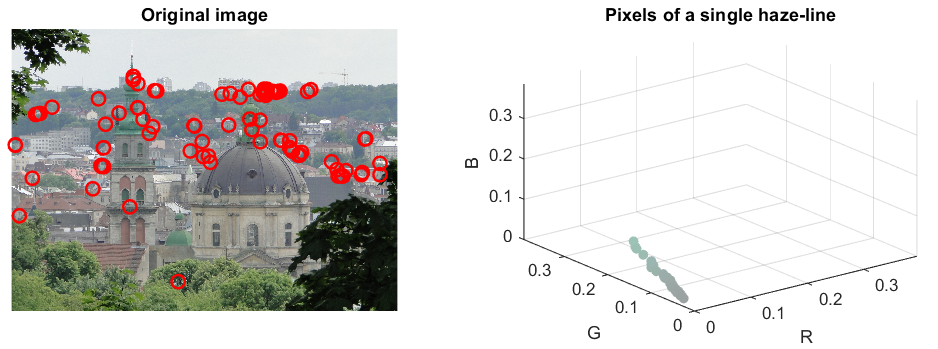
\includegraphics[width=\linewidth]{img/hazeLine.png}
    \caption{Haze-line example of an image. The red circles in the original image (left) are the pixels of the haze line. The right plot shows the same pixels in an RGB space centered around the airlight vector.}
    \label{fig:haze_lines}
\end{figure}
The transmission $t(\mathbf{x})$ is approached by estimating the dominant colour of each haze-line as the one of the pixels with the highest distance to the airlight vector:
\begin{equation}
    \label{eq:dominant_color}
    r_{max, H} = \max_{\mathbf{x} \in H} r(\mathbf{x})
\end{equation}
Where $H$ is the haze-line. The transmission coefficient estimate $\tilde{t}(\mathbf{x})$ is then computed as the ratio between the distance of the pixel to the airlight vector $r(\mathbf{x})$ and the maximum distance of the haze-line $r_{max, H}$:
\begin{equation}
    \label{eq:transmission_estimate}
    \tilde{t}(\mathbf{x}) = r(\mathbf{x})/r_{max, H}
\end{equation}
This transmission coefficient estimate has a lower bound of $t_{LB}(\mathbf{x})$, which is defined in \cite{dehaze} as:
\begin{equation}
    \label{eq:lower_bound_transmission}
    t_{LB}(\mathbf{x}) = 1 - \min_{c \in \{R, G, B\}} \left\{I_c(\mathbf{x}) / A_c\right\}
\end{equation}
This lower bound is used to ensure that the radiance $\mathbf{J}$ is not negative.\par
Using this estimate $\tilde{t}$ would not be very efficient as it would lead to a transmission coefficient that is not continuous across the image. Fig. \ref{fig:first_transmission} shows the transmission coefficient computed using the method described above together with the reference image.\par
\begin{figure}
    \centering
    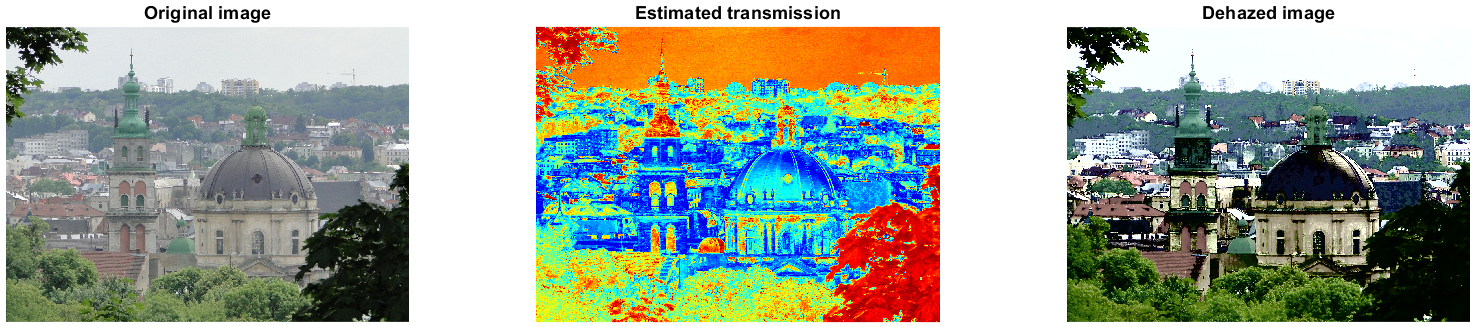
\includegraphics[width=\linewidth]{img/noOpti.png}
    \caption{First transmission estimate. The left image is the original image and the transmission coefficient estimate is on the right.}
    \label{fig:first_transmission}
\end{figure}
To have a smoother transmission coefficient, the authors of \cite{dehaze} propose to apply an optimization algorithm that aims to find $\hat{t}(\mathbf{x})$ that minimizes:
\begin{equation}
    \label{eq:cost_function}
    C(\tilde{t}) = \sum_{\mathbf{x}} \frac{\left[\hat{t}(\mathbf{x}) - \tilde{t}(\mathbf{x})\right]^2}{\sigma^2(\mathbf{x})} + \lambda \sum_{\mathbf{x}} \sum_{\mathbf{y} \in N_{\mathbf{x}}} \frac{\left[\hat{t}(\mathbf{x}) - \hat{t}(\mathbf{y})\right]^2}{||\mathbf{I}(\mathbf{x}) - \mathbf{I}(\mathbf{y})||^2}
\end{equation}
Where $\sigma(\mathbf{x})$ is the standard deviation of $r(\mathbf{x})$ for $\mathbf{x} \in H$, $\lambda$ is a parameter that controls the importance of the smoothness of the transmission coefficient and $N_{\mathbf{x}}$ is the set of pixels in a $3 \times 3$ neighbourhood of $\mathbf{x}$.\\
The first term of the cost function Eq. (\ref{eq:cost_function}) keeps the transmission coefficient close to the estimate $\tilde{t}(\mathbf{x})$. The second term penalizes differences between the transmission coefficient of neighbouring pixels, thus enforcing the smoothness constraint. 
The optimization is done using a weighted least squares optimizer provided in \cite{github}. The weights are chosen in a way that penalizes haze-lines with a low number of pixels, which avoids such haze-lines to have a large influence on the final transmission coefficient. The weights also depends on the standard deviation of $r(\mathbf{x})$ to give less importance to haze-lines with a large spread. \par
The optimal transmission coefficient $\hat{t}(\mathbf{x})$ is then computed with $\lambda = 0.1$ and gives a smooth transmission coefficient as shown in Fig. \ref{fig:final_transmission}. 
\begin{figure}
    \centering
    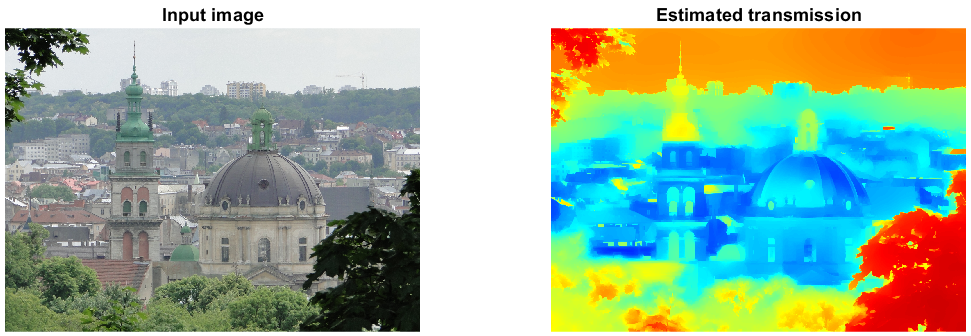
\includegraphics[width=\linewidth]{img/opti.png}
    \caption{Final transmission estimate.  The left image is the original image and the transmission coefficient estimate, after optimization, is on the right.}
    \label{fig:final_transmission}
\end{figure}
The final step is to recover the true radiance $\mathbf{J}(\mathbf{x})$ using the computed transmission coefficient and the airlight vector with Eq. (\ref{image_model}):
\begin{equation}
    \mathbf{J}(\mathbf{x}) = \frac{\mathbf{I}(\mathbf{x}) - (1 - \hat{t}(\mathbf{x})) \cdot \mathbf{A}}{\hat{t}(\mathbf{x})}
\end{equation}

\section{Validation}
The whole algorithm has been used on several images as can be seen in Fig. (\ref{validation1}, \ref{validation2}, \ref{validation3}).
\begin{figure}
    \centering
    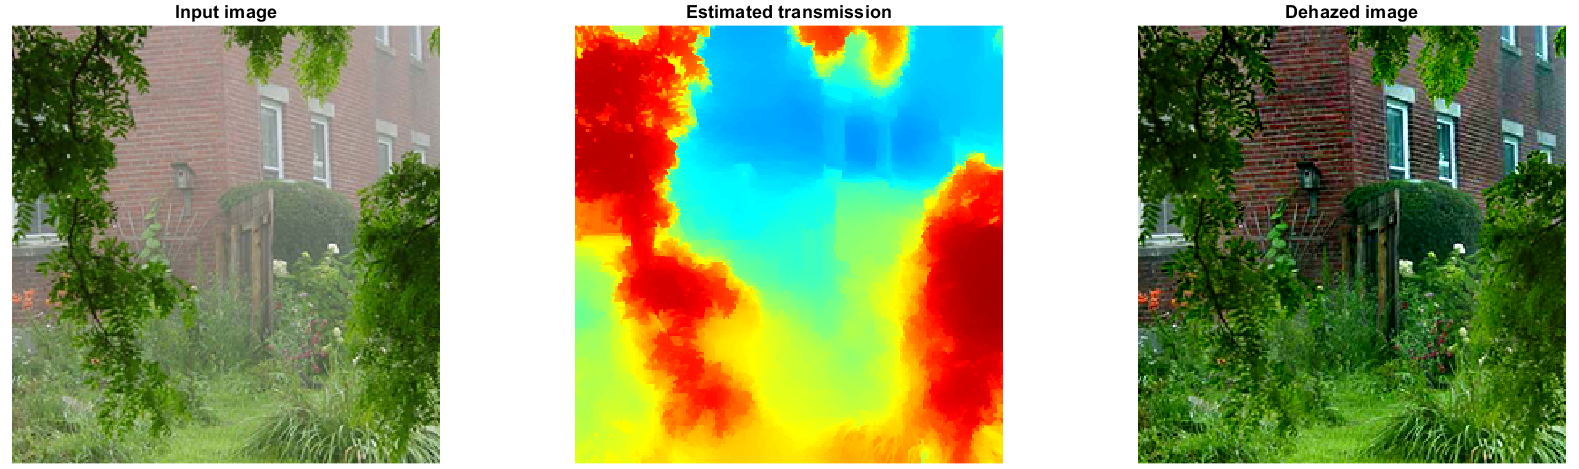
\includegraphics[width=\linewidth]{img/validation1.png}
    \caption{Validation of the dehazing algorithm on an image. The left image is the original image, the middle one is the transmission coefficient and the right one is the dehazed image.}
    \label{validation1}
\end{figure}
\begin{figure}
    \centering
    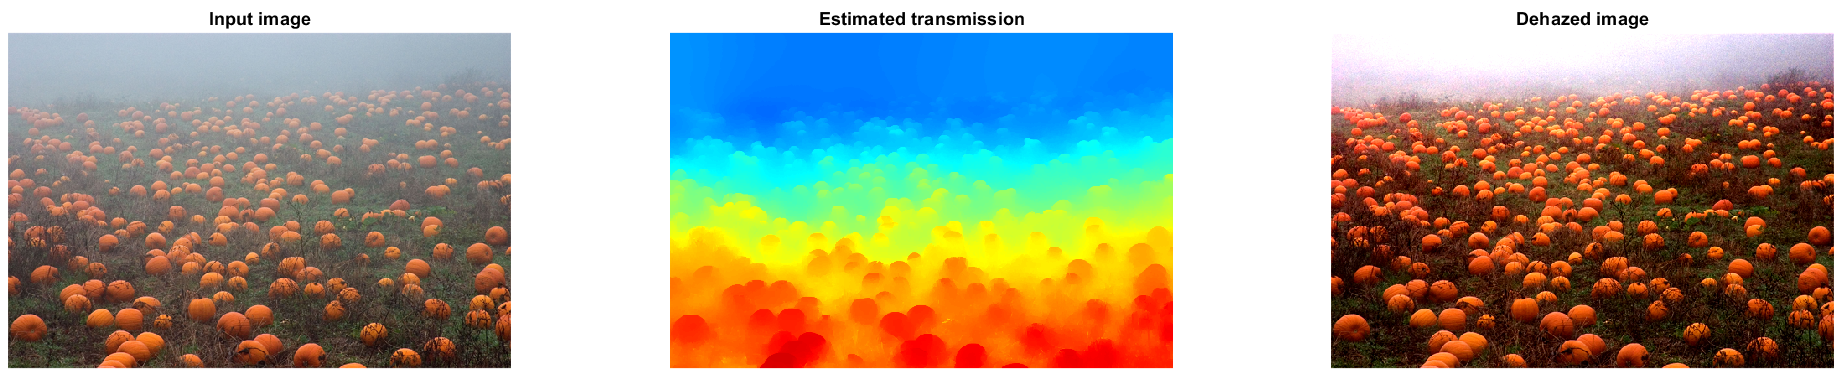
\includegraphics[width=\linewidth]{img/validation2.png}
    \caption{Validation of the dehazing algorithm on an image. The left image is the original image, the middle one is the transmission coefficient and the right one is the dehazed image.}
    \label{validation2}
\end{figure}
\begin{figure}
    \centering
    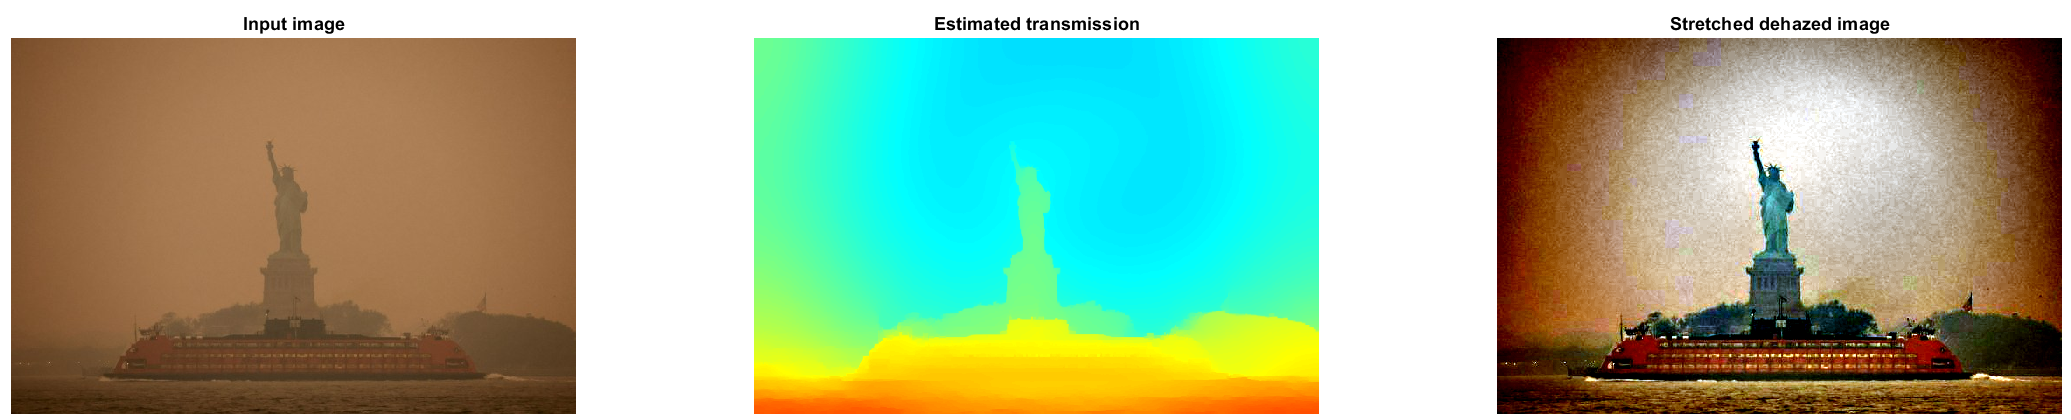
\includegraphics[width=\linewidth]{img/validation3.png}
    \caption{Validation of the dehazing algorithm on an image. The left image is the original image, the middle one is the transmission coefficient and the right one is the dehazed image on which a histogram stretching has been applied.}
    \label{validation3}
\end{figure}
Fig. \ref{validation3} shows that the algorithm is able to work even for images with a lot of haze. Insterad of removing haze, we can also increase it by applying Eq. (\ref{image_model}) in which the transmission coefficient is multiplied by a factor smaller than 1. This is shown in Fig. \ref{denser_haze} where the transmission coefficient is multiplied by 0.5.
\begin{figure}
    \centering
    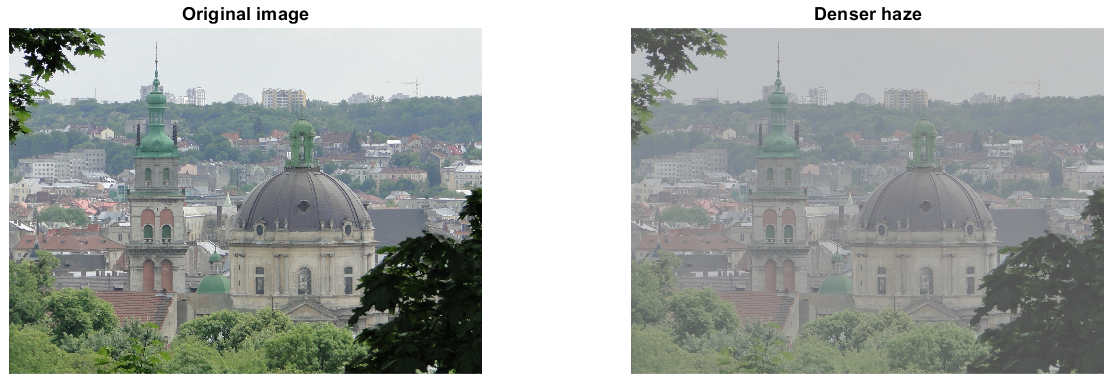
\includegraphics[width=\linewidth]{img/denser_haze.png}
    \caption{Increasing the haze of an image. The left image is the original image and the right one is the dehazed image with a denser haze.}
    \label{denser_haze}
\end{figure}
Another use of this algorithm is to estimate the distance of the scene points from the camera. This can be done by using Eq. (\ref{scattering_coefficient}) in which the distance $d(\mathbf{x})$ is computed as:
\begin{equation}
    d(\mathbf{x}) = -\frac{\ln(\hat{t}(\mathbf{x}))}{\beta}
\end{equation}
where $\beta$ is the wave phase number. A distance mapping is shown in Fig. \ref{distance_mapping}.
\begin{figure}
    \centering
    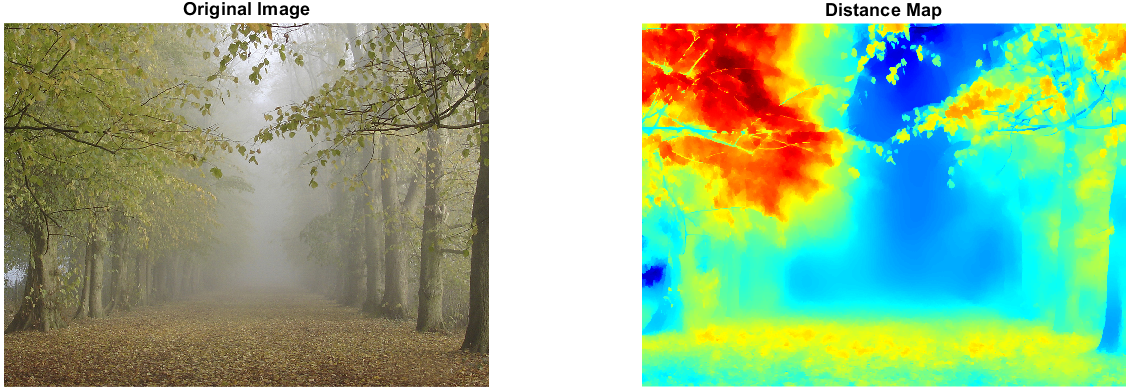
\includegraphics[width=\linewidth]{img/distance_mapping.png}
    \caption{Distance mapping of the scene points. The left image is the original image and the right one is the distance mapping.}
    \label{distance_mapping}
\end{figure}

\section{Conclusion}


\vspace{12pt}

\begin{thebibliography}{00}
\bibitem{airlight} M. Sulami, I. Glatzer, R. Fattal and M. Werman, "Automatic recovery of the atmospheric light in hazy images," 2014 IEEE International Conference on Computational Photography (ICCP), Santa Clara, CA, USA, 2014, pp. 1-11.
\bibitem{dehaze} D. Berman, T. Treibitz and S. Avidan, "Non-local Image Dehazing," 2016 IEEE Conference on Computer Vision and Pattern Recognition (CVPR), Las Vegas, NV, USA, 2016, pp. 1674-1682.
\bibitem{github}
D. Berman, non-local-dehazing, GitHub repository, 2018. [Online]. Available: \url{https://github.com/danaberman/non-local-dehazing}. [Accessed: May 31, 2025].
\end{thebibliography}

\end{document}
